\section{Fully dynamic \textit{k}-center clustering using navigating nets}


In this section, we present a fully-dynamic algorithm for the \textit{k}-center clustering problem that achieves a $(2 + \varepsilon)$-approximation with a running time not depending on the number of clusters $k$. The first component of our algorithm is to use a nearest neighbor search data structure called “navigating nets” (Krauthgamer and Lee \cite{krauthgamer2004navigating}). Unfortunately, this technique by itself only guarantees an 8-approximation, which does not suffice to obtain the claimed $(2 + \varepsilon)$-approximation factor. The second part of our construction is a seemingly unrelated scaling argument by McCutchen and Khuller \cite{mccutchen2008streaming} used in the context of incremental streaming algorithms. Our work is the first to apply this argument together with the nearest neighbor search data structures.

We start by reviewing notation from \cite{krauthgamer2004navigating}. 

\textit{r-\textbf{\text{net}}}. Let $(X, d)$ be a metric space. For a given parameter $r > 0$, a subset $Y_r \subseteq X$ is an \textit{r-net} of $X$ if the following properties hold:

\begin{enumerate}
    \item (separating) Distinct $x, y \in Y_r$ have $d(x, y) \geq r$.
    \item (covering) $X \subseteq \bigcup_{y \in Y_r} B(y, r)$.
\end{enumerate}

    \subsection{Navigating Nets}  
    Given a metric space $(M, d)$ which evolves over time with parameters $d_{\text{min}}$ and $d_{\text{max}}$, we define $\Gamma := \{\alpha^i : i \in \mathbb{Z}\}$ as the set of scales of $(M, d)$ for some $\alpha > 1$. We define an \textit{r}-net for all $r \in \Gamma$ as follows: For all $r < d_{\text{min}}$, we define $Y_r := M$ as a trivial $r$-net of $M$. For $r > d_{\text{min}}$, define $Y_r$ to be an $r$-net of $Y_{r/\alpha}$. Note that $Y_r$ is a subset of $Y_{r/\alpha}$ and contains a point with distance $\leq r$ to every point in $Y_{r/\alpha}$. 
    
    A navigating net $\Pi$ is defined as the union over all $Y_r$ for $r \in \Gamma$. We refer to the elements in $Y_r$ as centers. Note that for every scale $r > d_{\text{max}}$, the set $Y_r$ contains only one element due to the separating property. A navigating net $\Pi$ keeps track of (i) the smallest scale $r_{\text{max}}$ defined by $r_{\text{max}} = \min\{r \in \Gamma : \forall r' \geq r, |Y_{r'}| = 1\}$, and (ii) the largest scale $r_{\text{min}}$ defined by $r_{\text{min}} = \max\{r \in \Gamma : r' \leq r, Y_{r'} = M\}$. All scales $r \in \Gamma$ such that $r \in [r_{\text{min}}, r_{\text{max}}]$ are referred to as nontrivial scales. Figure \ref{fig:navigating_net_example} illustrates an example of a navigating net.


    \begin{figure}[h]
    \centering
    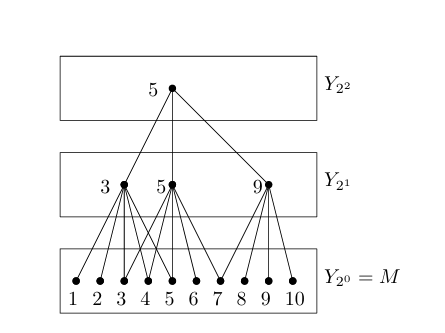
\includegraphics[width=0.5\linewidth]{graph.png} % Replace with the actual image file   
    \caption{An example for a navigating net with $M = \{1, 2, 3, 4, 5, 6, 7, 8, 9, 10\}$ where $d$ is Euclidean and $\alpha = 2$. Consequently, $\Gamma = \{2^i : i \in \mathbb{Z}\}$. In the navigating net, the nontrivial scales are given by $\{2^0, 2^1, 2^2\}$. Consequently, $r_{\text{max}} = 2^2$, $r_{\text{min}} = 2^0$.}
    \label{fig:navigating_net_example}
    \end{figure}

